\hypertarget{CartesianToPolarConverter_8cpp}{\section{src/multiscale/video/circular/\-Cartesian\-To\-Polar\-Converter.cpp File Reference}
\label{CartesianToPolarConverter_8cpp}\index{src/multiscale/video/circular/\-Cartesian\-To\-Polar\-Converter.\-cpp@{src/multiscale/video/circular/\-Cartesian\-To\-Polar\-Converter.\-cpp}}
}
{\ttfamily \#include \char`\"{}multiscale/exception/\-Cartesian\-To\-Polar\-Converter\-Exception.\-hpp\char`\"{}}\\*
{\ttfamily \#include \char`\"{}multiscale/video/circular/\-Cartesian\-To\-Polar\-Converter.\-hpp\char`\"{}}\\*
{\ttfamily \#include \char`\"{}multiscale/video/circular/\-Polar\-Gnuplot\-Script\-Generator.\-hpp\char`\"{}}\\*
{\ttfamily \#include \char`\"{}multiscale/util/\-Numeric\-Range\-Manipulator.\-hpp\char`\"{}}\\*
{\ttfamily \#include $<$iostream$>$}\\*
{\ttfamily \#include $<$fstream$>$}\\*
{\ttfamily \#include $<$exception$>$}\\*
{\ttfamily \#include $<$cassert$>$}\\*
{\ttfamily \#include $<$vector$>$}\\*
Include dependency graph for Cartesian\-To\-Polar\-Converter.\-cpp\-:\nopagebreak
\begin{figure}[H]
\begin{center}
\leavevmode
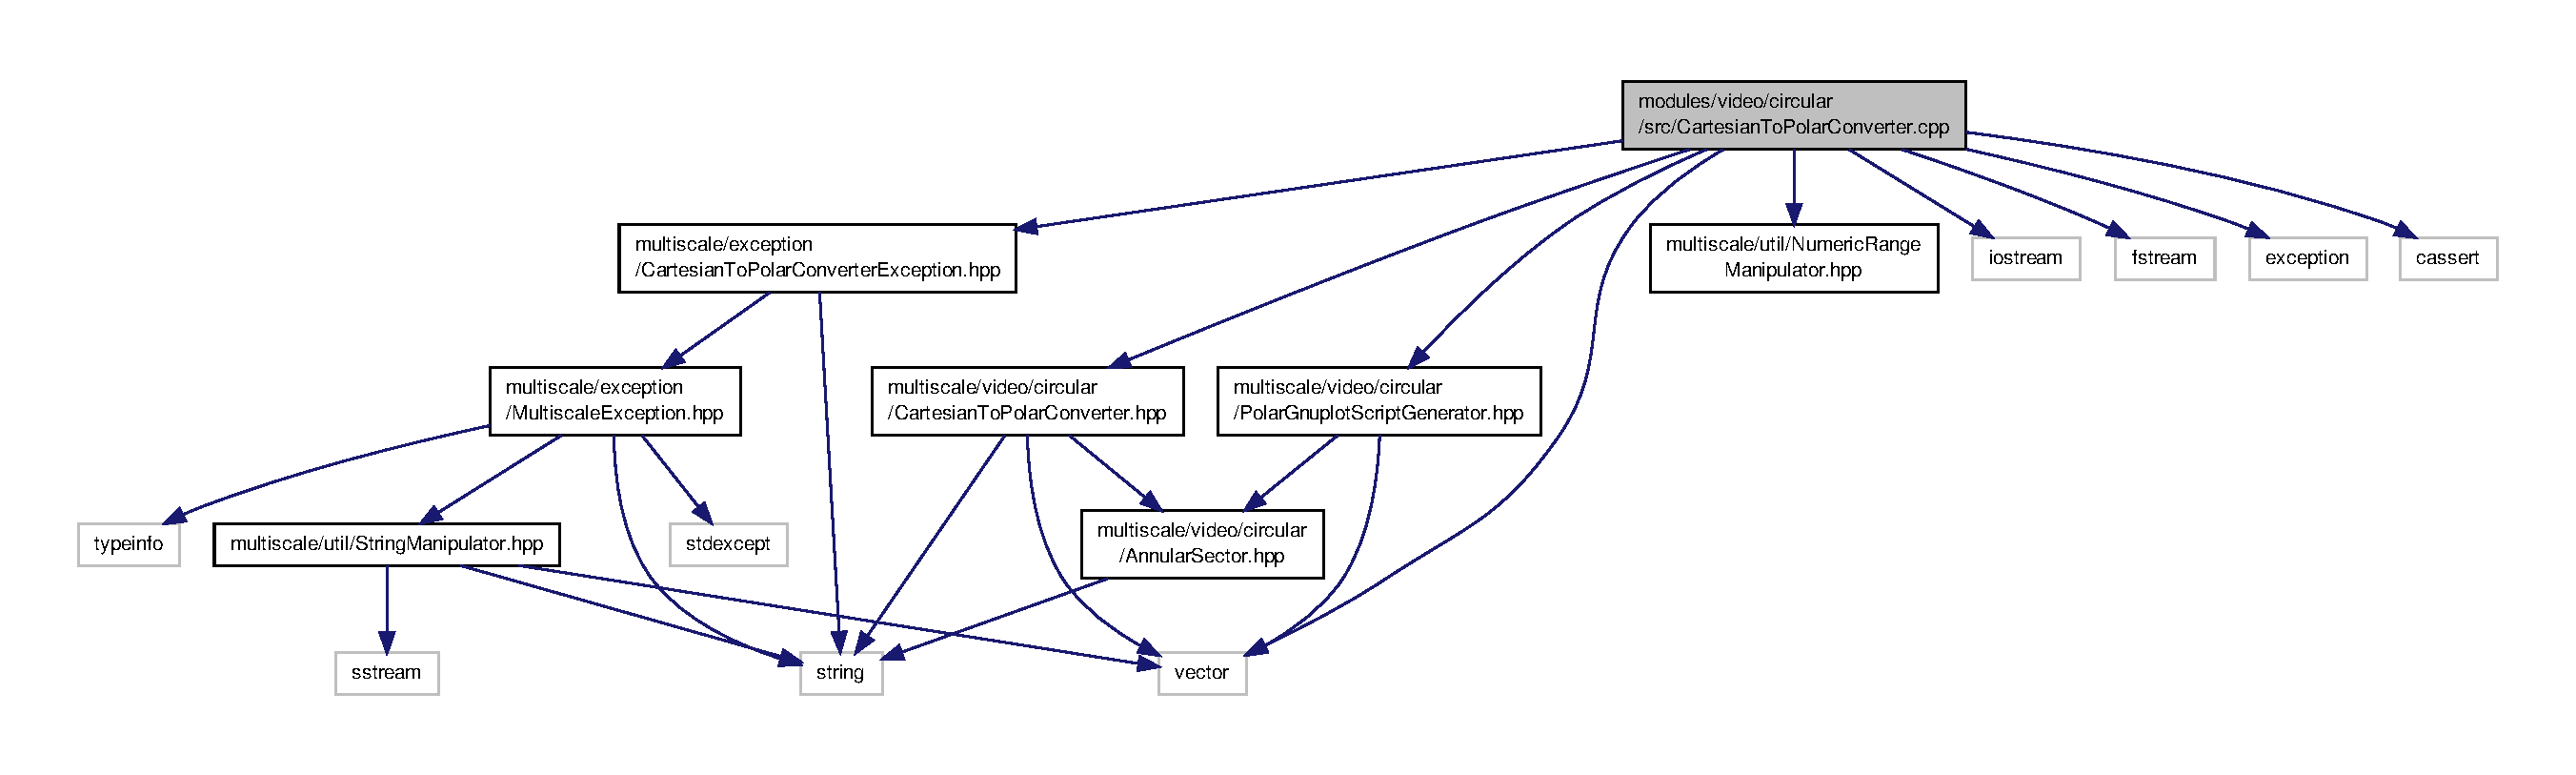
\includegraphics[width=350pt]{CartesianToPolarConverter_8cpp__incl}
\end{center}
\end{figure}
